%! TeX program = lualatex
\documentclass[a4paper,11pt]{article} 
% packages
\usepackage{fontspec}
\setmainfont{EB Garamond}
% for tironian et fallback
% % \directlua{luaotfload.add_fallback
% % ("emojifallback",
% %      {"Noto Serif:mode=harf"}
% % )}
% % \setmainfont{EB Garamond}[RawFeature={fallback=emojifallback}]

\setmonofont[Scale=MatchLowercase]{Deja Vu Sans Mono}
\usepackage[a4paper,left=2cm,right=2cm,top=\dimexpr15mm+1.5\baselineskip,bottom=2cm]{geometry}
\setlength{\parindent}{0pt}

\usepackage{fancyhdr}       % Headers and footers 
\fancyhead[R]{\normalfont \leftmark}
\fancyhead[L]{}
\pagestyle{fancy}

\usepackage{microtype}      % Slightly tweak font spacing for aesthetics
\usepackage[english]{babel} % Language hyphenation and typographical rules
\usepackage[final, colorlinks = false, urlcolor = cyan]{hyperref} 
\usepackage{xurl}
\usepackage{changepage}     % adjust margins on the fly

\usepackage{minted}
\usemintedstyle{algol_nu}
\usepackage{xcolor}

\usepackage{pgfplots}
\pgfplotsset{width=\textwidth,compat=1.9}

\usepackage{caption}
\newenvironment{code}{\captionsetup{type=listing}}{}
\captionsetup[listing]{skip=0pt}
\setlength{\abovecaptionskip}{5pt}
\setlength{\belowcaptionskip}{5pt}

\usepackage[yyyymmdd]{datetime}
\renewcommand{\dateseparator}{--}

\renewcommand{\labelenumii}{\arabic{enumi}.\arabic{enumii}}

\usepackage{titlesec}

\author{Andrew Hayes}

\begin{document}
\begin{titlepage}
    \begin{center}
        \hrule
        \vspace*{0.6cm}
        \huge \textbf{CT3536: Games Programming}
        \vspace*{0.6cm}
        \hrule
        \LARGE
       \vspace{0.5cm}
       Project Report
       \vspace{0.5cm}
       \hrule
            
       \vfill
       % 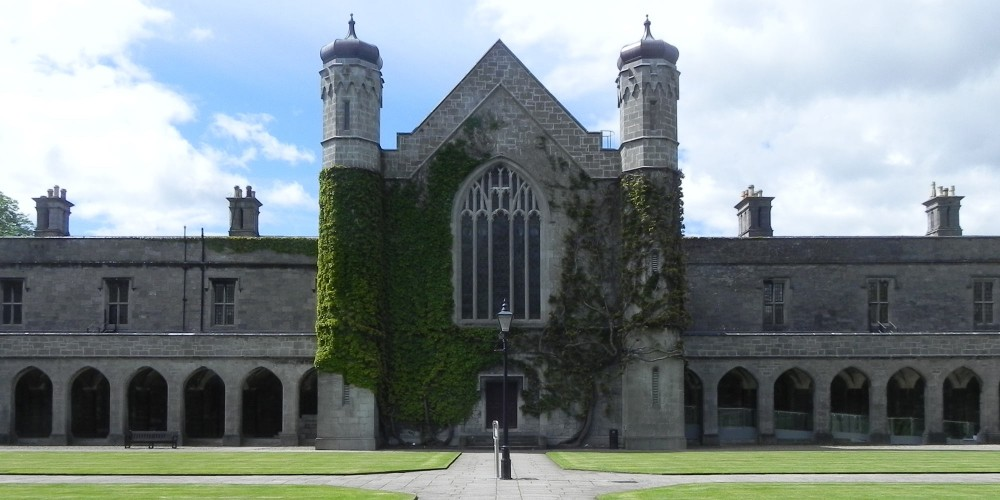
\includegraphics[width=\textwidth]{images/uniog.jpg}
        \vfill

        \Large
       \vspace{0.5cm}
       \hrule
       \vspace{0.5cm}
       \textbf{Andrew Hayes}
       % \vspace{0.5cm}
       % \hrule
       % \vspace{0.5cm}
            
       \normalsize
       Student ID: 21321503

       % \today

       \vspace{0.5cm}
       \hrule
    \end{center}
\end{titlepage}

\pagenumbering{roman}
\newpage
\tableofcontents
\newpage
\setcounter{page}{1}
\pagenumbering{arabic}

\section{Introduction \& Instructions}
This game is a single-player racing game in which the player races against a computer-controlled car on a race track.
Each race consists of 3 laps, with the first ``player'' (i.e. the actual player or the computer-controlled car) to cross the finish
line being declared the winner.
All in all, the game is quite self-explanatory: it's a player vs computer car racing game, with the usual controls and behaviours
one would expect.
All of the art and sound assets in this game were originally sourced from a third party and were not created by me, although 
adjustments and edits were made to suit my use case.

\begin{figure}[H]
    \centering
    \includegraphics[width=\textwidth]{~/media/images/screenshots/2024-01-07 20:55:45.png}
    \caption{Starting Point of Game}
\end{figure}

The main menu consists of the options ``Start Game'' or ``Quit''.
When a race is started, the track and cars appear, but are immobile until the race has started.
Three air horns are sounded at one second intervals to count down to the race start, followed by an air horn to indicate ``Go''.
From there, the \verb|WASD| keys can be used to control the player car to drive it around the track, by turning its wheel colliders 
to push it forward.

\begin{figure}[H]
    \centering
    \includegraphics[width=\textwidth]{~/media/images/screenshots/2024-01-07 20:55:38.png}
    \caption{Start Menu}
\end{figure}

The computer-controlled car travels between a set of waypoints on the track. 
To give the player an edge over the computer, the NPC car will stop if it is on a collision course with the player's car, i.e. 
if the player's car is both close to and directly in from of the computer-controlled car.
\\\\
The game ends when one ``player'' has completed three laps.
When the game ends, the player is sent back to the main menu, and a message is displayed indicating whether they won or lost.

\begin{figure}[H]
    \centering
    \includegraphics[width=\textwidth]{~/media/images/screenshots/2024-01-07 21:02:29.png}
    \caption{``Win'' Screen}
\end{figure}

\section{Development Approach}
The first thing I did when I decided to start developing a racing game was to look for a free racing car prefab 
that I could use, and the first one that appeared on the Unity asset store seemed ideal:

\begin{figure}[H]
    \centering
    \includegraphics[width=\textwidth]{~/media/images/screenshots/2024-01-07 22:02:20.png}
    \caption{Racecar Prefab}
\end{figure}

Originally, I was going to just apply a physics force to the car object to make it go forwards, but I noticed 
that this car asset came with individual colliders and transforms for each wheel, allowing them to be manipulated 
independently.
I later discovered that this was standard practice for cars in Unity, and the rotation of the wheel was 
typically used to propel the car. 
As this was definitely better than just applying a physics force to the back of the car, I opted to use the 
wheel rotation to propel the car.
A mistake that I made here was to make the car front-wheel drive: as I don't drive myself, I just picked one 
at random when I was developing, ignorant of how uncommon it was for race cars to be front-wheel drive. 
The plus side of this was that it made the car lend itself quite easily to ``drifting''-like motions.
\\\\
When it came to making the main camera follow the car, I had a lot of trouble getting the camera to realise that 
the car's position had changed. 
For some reason, no matter what changes I made, the camera seemed to think that the player's car was always at 
(0,0,0).
To get around this problem easily, I instead decided to make the car summon the camera to it, which ensured that 
the camera was always getting updated as the car's position changed.
The drawback of this was that it led to less clean code architecture: the camera was being controlled by a script 
that was not attached to it, meaning that if I wanted to expand the game to allow the camera to move around to 
view other things than the car, development would be difficult.
However, since I didn't plan on doing that for this project, I was prepared to sacrifice some code structure for 
quickly working code.
\\\\
To get the car to make motor noises as one would expect, I initially considered getting several different car engine 
noise samples at different RPMs and mixing between them as appropriate. 
However this struck me as needlessly complicated, and it was prohibitively difficult to find a set of free-to-use
engine noise samples that also looped cleanly: it proved difficult enough to find one decent engine noise sample.
Instead, I decided to use one engine noise sample that would loop endlessly, and to just pitch it up or down 
to correspond the to the hypothetical ``revs'' of the engine.
I still found it difficult to find a clean, looping sample of a car engine, but I eventually found one that was
``close enough''.
It didn't loop perfectly though, so I edited it using Audacity to make it shorter, get rid of the silence, etc.

\begin{figure}[H]
    \centering
    \includegraphics[width=\textwidth]{~/media/images/screenshots/2024-01-07 22:17:38.png}
    \caption{Editing the Engine Noise Sample in Audacity}
\end{figure}

To design the racetrack structure, I made use of a tool called RoadArchitect which provides a number of 
road structure prefabs and allows you to configure them into a road system consisting of several nodes.
To avoid any confusion, I want to state clearly here that this tool does not execute code during the game loop 
nor is any of its code included in my game: a static road structure was created and designed using this tool, 
which is then used as a (code-free) GameObject in the game.

\begin{figure}[H]
    \centering
    \includegraphics[width=0.8\textwidth]{~/media/images/screenshots/2024-01-07 22:25:08.png}
    \caption{Racetrack Structure}
\end{figure}

The node-based structure of the road proved to be useful for creating the computer-controlled car; the car 
navigates the track by heading towards a series ``waypoints'', many of which are the nodes of the road itself.
To make the race more interesting, the player is afforded an advantage: it can force the computer-controlled car
to stop if the computer-controlled car is about to collide with it. 
To make this possible, the computer-controlled car is constantly casting rays out in its forward direction and 
checking to see if they hit any objects tagged ``Player'': if they do, it does not proceed until its raycasts 
are not hitting the player.
These raycasts are limited to a short distance so as not to render the computer-controlled car entirely helpless.
\\\\
Finally, different touches were added to the game to make it more cohesive: trees were painted, terrain was
moulded, and horn \& buzzer sound effects were added to the countdown before the race begins.
A main menu was added which allows the player to quit or race again, which also doubles as the announcement area 
of whether the player won or lost the race.

\section{Source Code}
\begin{code}
\inputminted[texcl, mathescape, linenos, breaklines, frame=single]{csharp}{../Assets/EngineSound.cs}
\caption{\texttt{EngineSound.cs}}
\end{code}

\begin{code}
\inputminted[texcl, mathescape, linenos, breaklines, frame=single]{csharp}{../Assets/GameManager.cs}
\caption{\texttt{GameManager.cs}}
\end{code}

\begin{code}
\inputminted[texcl, mathescape, linenos, breaklines, frame=single]{csharp}{../Assets/LapDisplay.cs}
\caption{\texttt{LapDisplay.cs}}
\end{code}

\begin{code}
\inputminted[texcl, mathescape, linenos, breaklines, frame=single]{csharp}{../Assets/NPCCar.cs}
\caption{\texttt{NPCCar.cs}}
\end{code}
 
\begin{code}
\inputminted[texcl, mathescape, linenos, breaklines, frame=single]{csharp}{../Assets/PlayerCar.cs}
\caption{\texttt{PlayerCar.cs}}
\end{code}
 
\begin{code}
\inputminted[texcl, mathescape, linenos, breaklines, frame=single]{csharp}{../Assets/QuitGame.cs}
\caption{\texttt{QuitGame.cs}}
\end{code}
 
\begin{code}
\inputminted[texcl, mathescape, linenos, breaklines, frame=single]{csharp}{../Assets/StartRace.cs}
\caption{\texttt{StartRace.cs}}
\end{code}
 
\begin{code}
\inputminted[texcl, mathescape, linenos, breaklines, frame=single]{csharp}{../Assets/SummonCamera.cs}
\caption{\texttt{SummonCamera.cs}}
\end{code}

\section{Third Party Assets Used}
Below is a list of all third party art assets that I used in this project:
\begin{itemize}
    \item   Grass textures: \url{https://assetstore.unity.com/packages/2d/textures-materials/floors/hand-painted-grass-texture-78552}
    \item   Racecar prefabs: \url{https://assetstore.unity.com/packages/3d/vehicles/land/arcade-free-racing-car-161085}
    \item   Asphalt textures: \url{https://assetstore.unity.com/packages/2d/textures-materials/roads/asphalt-materials-141036}
    \item   Audio clip for engine noises: \url{https://pixabay.com/sound-effects/engine-6000/}
    \item   Road prefabs: \url{https://github.com/FritzsHero/RoadArchitect}
    \item   Image for finish line material: \url{https://www.deviantart.com/fantasystock/art/Beveled-Checker-Board-Seamless-15233976}
    \item   Audio clip for buzzer sound: \url{https://soundbible.com/1501-Buzzer.html}
    \item   Audio clip for airhorn sound: \url{https://soundbible.com/1542-Air-Horn.html}
    \item   Tree prefabs: \url{https://assetstore.unity.com/packages/3d/vegetation/trees/free-trees-103208}
    \item   Skybox prefabs: \url{https://assetstore.unity.com/packages/2d/textures-materials/sky/free-stylized-skybox-212257}
\end{itemize}

\end{document}
